\documentclass[12pt]{article}

% Import packages
\usepackage{listings}  % For adding C code
\usepackage{xcolor}    % For custom colors
\usepackage{graphicx}  % For including images
\usepackage{amsmath}   % For advanced math formatting
\usepackage{hyperref}  % For creating hyperlinks
\usepackage{geometry}  % To set page margins
\usepackage{subfig}
\usepackage{multicol}
\usepackage{float}
\geometry{a4paper, margin=1in}

\lstdefinestyle{cstyle}{
    language=C,
    basicstyle=\ttfamily\footnotesize,
    keywordstyle=\color{purple}\bfseries,
    stringstyle=\color{orange},
    commentstyle=\color{olive},
    numbers=none,                           % No line numbers
    tabsize=2,                              % Tab space width
    showspaces=false,
    showstringspaces=false,
    frame=single,                           % Adds a single-line box around the code
    framerule=0.8pt,                        % Thickness of the frame
    framesep=5pt,                           % Space between frame and code
}

\title{\textbf{ESPX - Crypto Analysis Project}}
\author{Savvas Tzanetis - 10889}
\date{Aug 2025}

\begin{document}

\maketitle

\section{Introduction}
    This report is part of an assignment for the \textbf{Real-Time Embedded Systems} class of the Aristotle University's 
    Electrical and Computer Engineering department.  \\

    This project implements real-time operations based on cryptocurrency prices that are updated every second. 
    It aims to make timely and accurate calculations, analyzing the cryptocurrency market, with the goal to assess 
    direct correlations between different cryptocurrencies. More specifically the project focus on the 8 different 
    cryptocurrencies that can seen in the list below and their evaluation in USDT.

    \begin{multicols}{4}
        \begin{itemize}
            \item BTC
            \item ADA
            \item ETH
            \item DOGE
            \item XRP
            \item SOL
            \item LTC
            \item BNB
        \end{itemize}
    \end{multicols}

    This document focuses on how raw data was captured and stored, the data analysis necessary to make correct evaluations, 
    to ensure long operation times as well as run in a Raspberry Pi, all in a timely fashion. The code for this project as 
    well as the \textit{Preparation assignment} can be seen in their 
    \textcolor{blue}{\href{https://github.com/stzanetis/ESPX-CryptoAnalysis}{GitHub repository}} page.

\section{System Methodology}
    In the proposed methodology, multiple threads were used for executing the different program processes. 
    A logger thread was created for receiving symbol data, While a processing thread was responsible for processing the received data every minute.

    \subsection{Cross-Compilation}
        For the project, a \textit{Raspberry Pi Zero 2W} was used, running a 64-bit version of \textit{Raspberry Pi OS lite}. 
        A binary was created using a pre-compiled cross compiler after copying the \textit{sysroot} from the Raspberry Pi with 
        every dependency pre-installed and statically linked. After the final executable was created, it was copied and executed 
        to the target system via \textit{ssh}. \\

        The binary was executed as a system process running on \textit{user space} via \textit{systemctl}. 
        This method proved to be a more robust option compared to \textit{nohup}, preventing program halting due to websocket 
        timeouts, and ensuring the correct operation of the program for the required 48 hours.

    \subsection{Data Collection}
        Using the \textbf{libwebsockets} library, we were able to open a websocket to the OKX public channel, 
        receiving data with minimal latency in a JSON format. The incoming JSON data was parsed using the \textbf{cjson} 
        library to a custom data structure. Lastly, parsed data was written in symbol-specific .log files. The written logs included the following data: 
        \[
            \text{[Timestamp], Price: [Value], Volume: [Volume]}
        \]
        Due to the nature of the websocket as well as the library used, regular ping/pong messages were needed to verify a healthy 
        connection with the OKX public channel. In addition, to ensure the longevity of the program, once a missed ping was interpreted, 
        an immediate attempt to reconnect was initialized with an exponential backoff, reducing wasted cycles and giving a chance for 
        the server to recover in case of an error. This process was executed entirely on a logger thread, ensuring uninterrupted execution, 
        logging incoming data with minimal delay.
        
    \subsection{Data Analysis}
        A processing thread is responsible for processing the parsed data collected from the logger thread every minute. This thread analyzed 
        the data, calculating a $15 minute$ moving average for each cryptocurrency symbol at the exact minute mark. For this calculation 
        a circular buffer was used to store the 8 most recent price points. \\

        In addition to the moving average calculation, the processor thread also calculated the Pearson correlation of every available 
        cryptocurrency symbol pair with the same frequency, using the previously calculated moving average of the last $8 minutes$(8 data points). 
        More specifically, given two series $x$ and $y$ representing the moving averages, the correlation was computed as:
        \[
            r =
            \frac{
                \sum_{i=1}^{n} x_i y_i - \tfrac{1}{n}\left(\sum_{i=1}^{n} x_i\right)\left(\sum_{i=1}^{n} y_i\right)
            }{
                \sqrt{
                    \left(\sum_{i=1}^{n} x_i^2 - \tfrac{1}{n}\left(\sum_{i=1}^{n} x_i\right)^2\right)
                    \left(\sum_{i=1}^{n} y_i^2 - \tfrac{1}{n}\left(\sum_{i=1}^{n} y_i\right)^2\right)
                }
            }
        \]

\section{Results Evaluation}
    In this section we will discuss the results of our methodology in terms of its timing delay when analyzing symbol data, 
    the CPU utilization of our Raspberry Pi Zero 2W when running our program, as well as the results of the moving average and 
    correlation calculations. These results were produced in a span of 48 hour continuous operation.

    \subsection{Data Analysis Delay}
        In Figure \ref{fig:proc_duration} we can see a graph of the duration of computing the moving average as well as correlation values. 
        Each vertical line represents one calculation that it self happened once every minute. As is visible, such calculation lasted an 
        average of $5ms~6ms$ with occasional spikes of up to $12ms$. These results indicate that these operation happened in a timely fashion, 
        without delaying the processing of new values as they were arriving, while the occasional spikes present could be attributed to websocket 
        reconnections.
        
        \begin{figure}[!h]
            \centering
            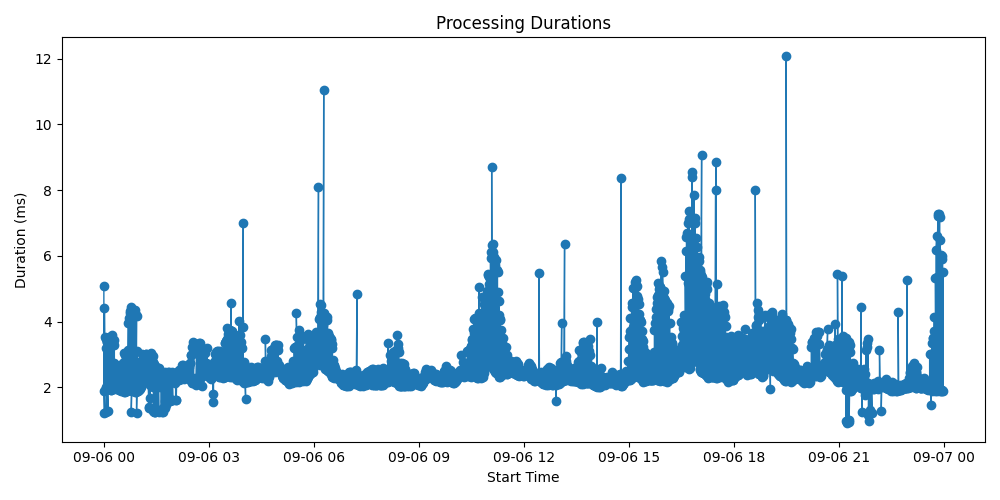
\includegraphics[width=0.8\linewidth]{../results/timings_durations.png}
            \caption{Processing Duration}
            \label{fig:proc_duration}
        \end{figure}
        
    \subsection{CPU Utilization}
        CPU utilization as seen in Figure \ref{fig:cpu_util} in average $0.5\%$. This indicates near negligible processing overhead. 
        Such behavior is expected and can be explained due to the fact that the Raspberry Pi Zero 2W has a quad-core processor in comparison 
        to its previous version were it had a single-core processor.
    
        \begin{figure}[!h]
            \centering
            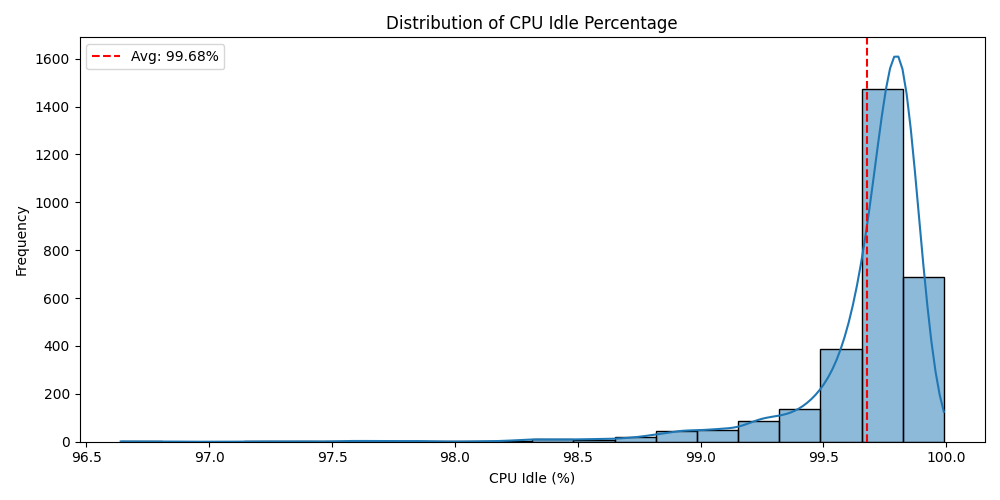
\includegraphics[width=0.8\linewidth]{../results/cpu_idle_histogram.png}
            \caption{CPU Utilization Histogram}
            \label{fig:cpu_util}
        \end{figure}

    \newpage
    \subsection{Calculated Metrics}
        Relatively strong correlation among all cryptocurrency symbols can be seen in the Figure \ref{fig:corr}'s heatmap as well the 
        moving average graphs of every symbol in Figure \ref{fig:mavg}.
        
        \begin{figure}[!h]
            \centering
            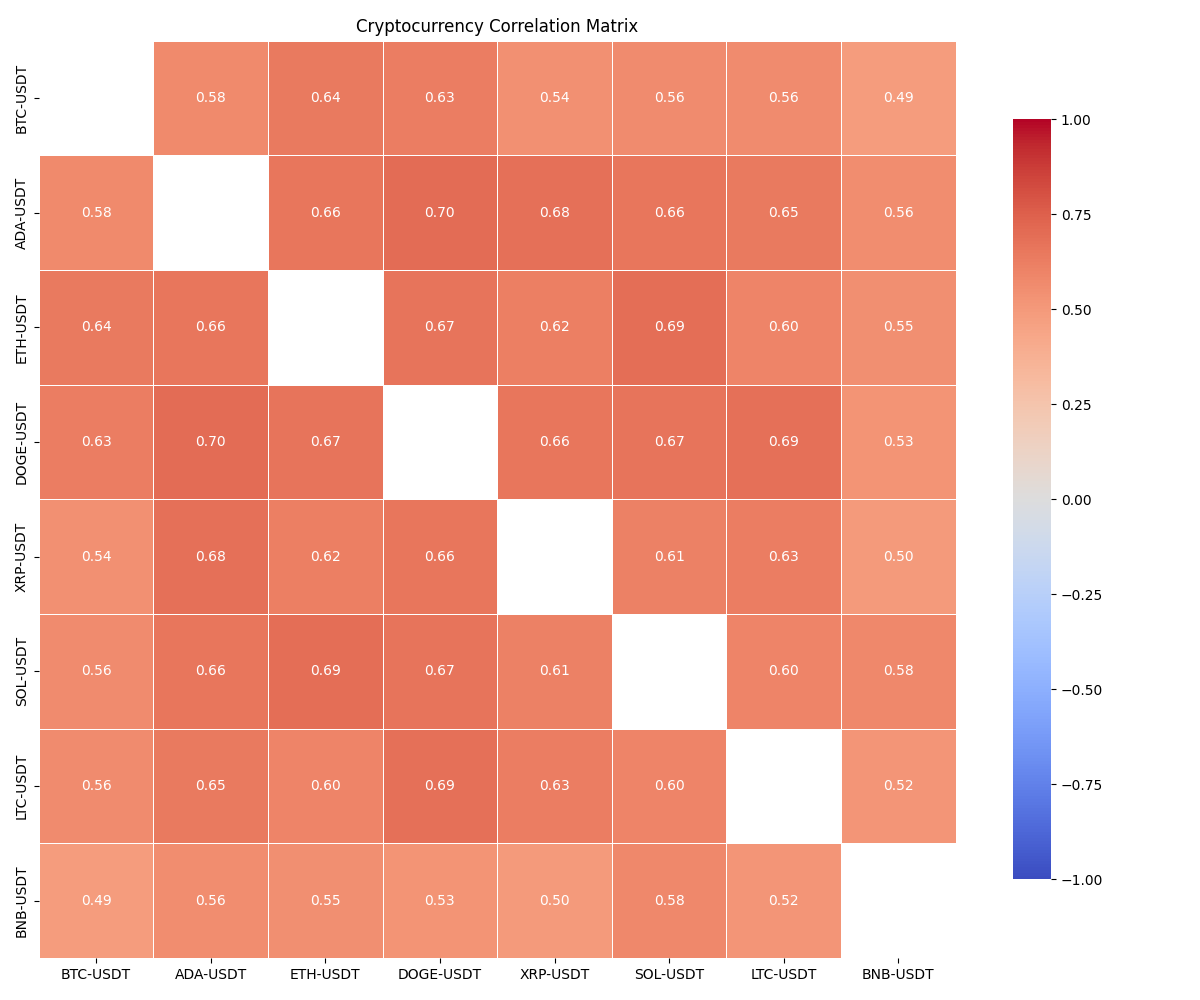
\includegraphics[width=0.7\linewidth]{../results/correlation_heatmap.png}
            \caption{Correlation Heatmap}
            \label{fig:corr}
        \end{figure}

        \begin{figure}[!h]
            \centering
            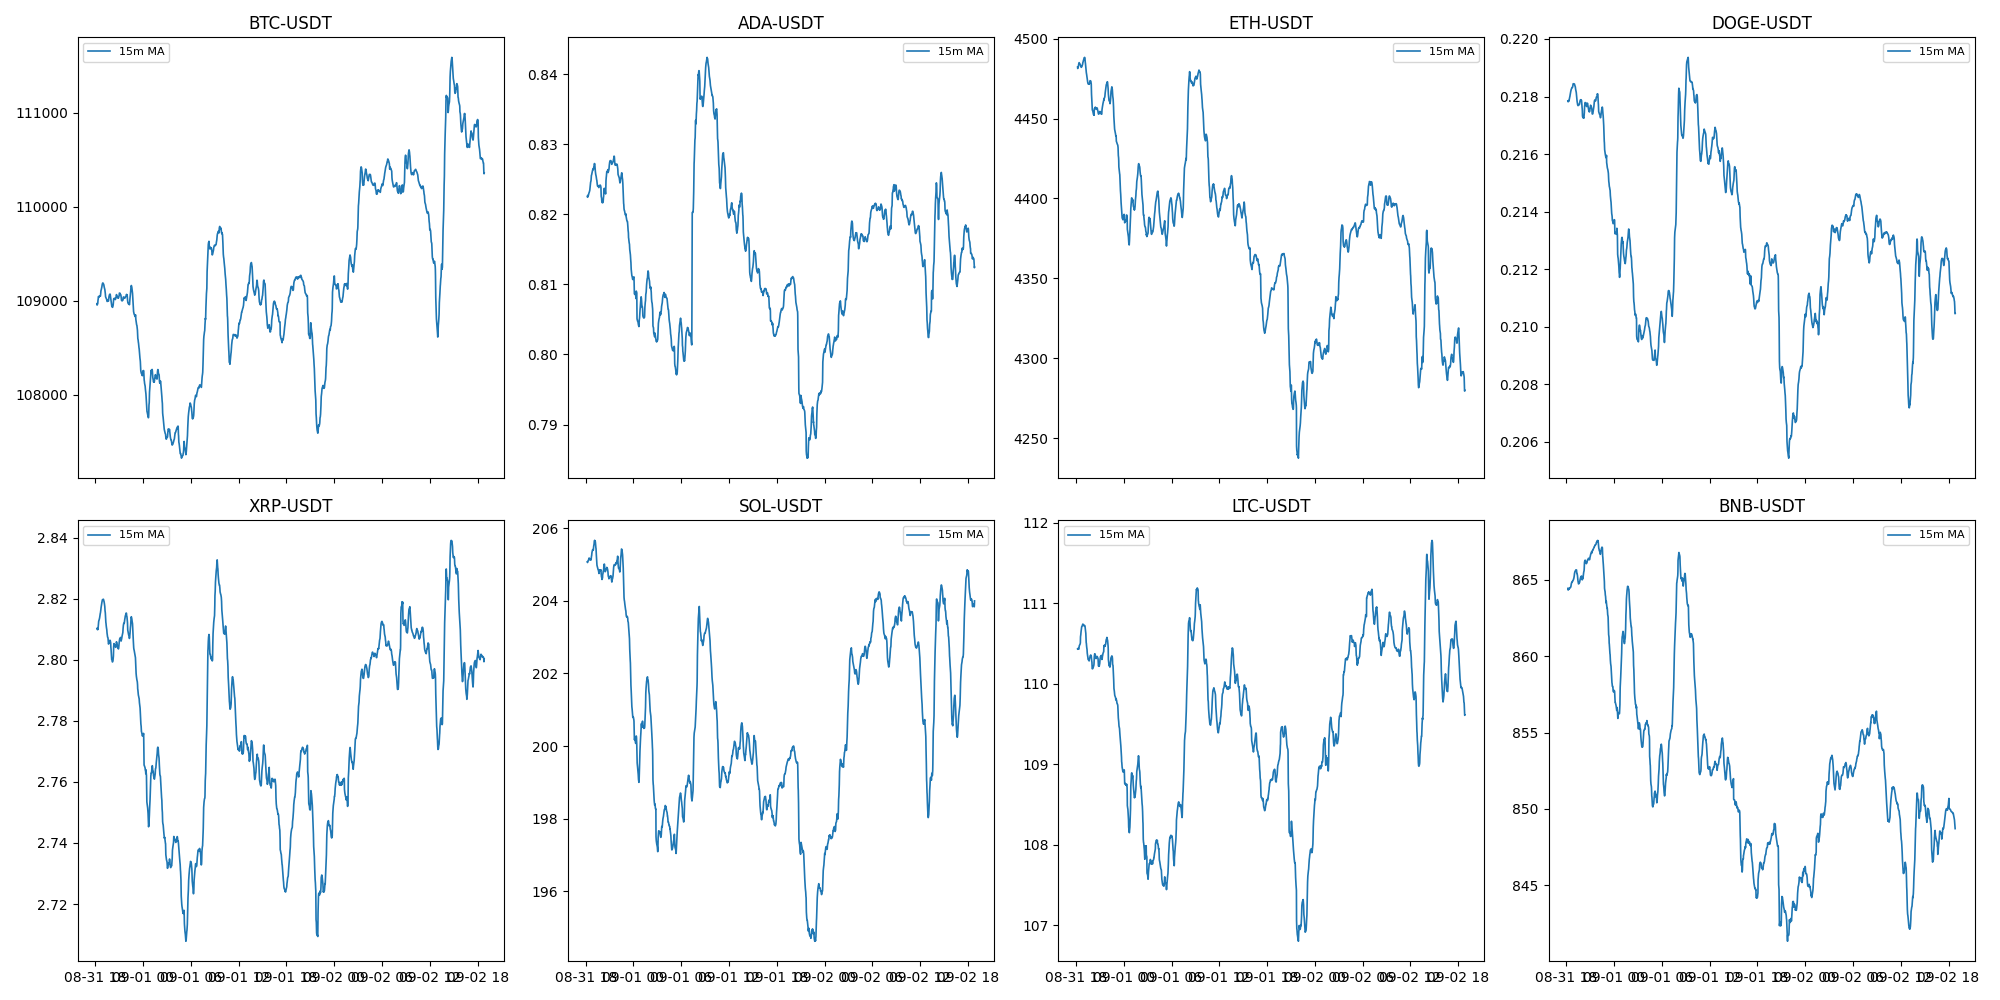
\includegraphics[width=0.7\linewidth]{../results/moving_averages.png}
            \caption{Moving Averages}
            \label{fig:mavg}
        \end{figure}
        
        Most notably, the highest correlation pairs are:
        \begin{itemize}
            \item \textbf{ADA - DOGE} with a 0.70 coefficient
            \item \textbf{ETH - SOL} with a 0.69 coefficient
            \item \textbf{DOGE - LTC} with a 0.69 coefficient
        \end{itemize}

        Though in general, similar coefficient values can be observed, suggesting a relatively high correlation amongst most cryptocurrency symbols tested.

\section{Conclusion}
    This project successfully implemented a real-time cryptocurrency analysis system aimed to run on low powered Raspberry Pi devices, 
    demonstrating that both data collection and processing can be performed efficiently with minimal latency. CPU utilization remained 
    near negligible, confirming the system's suitability for long-term operation on low-power hardware.

\section{Tools Used}
    In this project, the following tools where used:
    \begin{itemize}
        \item The \textbf{C} programming language.
        \item A \textbf{Raspberry Pi Zero 2W} running a lite version of \textbf{Raspbian OS}.
        \item \textbf{GitHub} for version control.
        \item \textbf{Python} for testing and results evaluation.
        \item The \textbf{libwebsockets} and \textbf{cjson} C programming libraries
        \item \textit{abhiTronix's} precompiled cross-compiler found in this \textcolor{blue}{\href{https://github.com/abhiTronix/raspberry-pi-cross-compilers/wiki/}{GitHub repository}} page
    \end{itemize}

\end{document}